\section{Calorimetry} \label{sec:atlas:calorimetry}

\begin{figure}[!htbp]
  \begin{center}
    \includegraphics[width=0.8\linewidth]{figures/atlas/calorimeter_cutaway}
    \caption{ \cite{PERF-2007-01} A cutaway diagram of ATLAS sampling calorimeters}
    \label{fig:calorimeter_cutaway}
  \end{center}
\end{figure}

Once the proton-proton collision remnants have passed through the ID and its
surrounding solenoid they enter into the ATLAS calorimeters depicted in
\Cref{fig:calorimeter_cutaway}.  Sampling calorimeter technologies were choosen
for their compact geometry and lower cost point.  These are constructed by
alternating layers of absorber, a dense material which reduces the incident
particles energy, and active material which produces a detectable signal when a
particle passes through.  This means that the detected signal is only a fraction
of the total energy of the particle and thus requires a study of the calorimeter
response for calibration purposes \cite{Fabjan:692252}. The first system, the
Electromagnetic Calorimeter (EMC), is designed to measure the energy of
electrons and photons which primarily lose their energy via bremsstrahlung and
pair production electromagnetic interactions.  Outside of the EMC is the
Hadronic Calorimeter (HCal) which is designed to measure the energy of jets of
hadrons through their electromagnetic and strong interactions. These detectors
cover the entire $|\eta| < 4.9$ range and provide complete containment of both
Electromagnetic and Hadronic showers with higher granularity in the EMC for
$|\eta| < 2.5$, the region matched to the ID, for precision measurements of
electrons and photons.  By instrumenting this huge space in $|\eta|$ we can
search for events with asymetric energy deposits which imply the existence of a
particle we didn't detect represented by missing transverse energy $\MET$.

\subsection{Electromagnetic Calorimeter}

The innermost calorimeter, the Liquid Argon (LAr) Electromagnetic Calorimeter
(EMC) \cite{PERF-2007-01}, uses Lead as the absorber and Liquid Argon as the
active material in an "accordion geometry" as seen in \Cref{fig:accordion}.
This geometry was chosen for uniform coverage in $\hat{\phi}$ due to its lack
of un-instrumented cracks in the radial direction.  The barrel region covers
$|\eta| < 1.475$ and an end cap on each side covers $1.375 < |\eta| < 3.2$ each
housed in their own cryostat.  The barrel is composed of two half barrels with
a 4mm gap at $z = 0$ and both end caps are divided into an inner wheel
covering $2.5 < |\eta| < 3.2$ and an outer wheel covering $1.375 < |\eta| <
2.5$.

\begin{figure}[!htbp]
  \begin{center}
    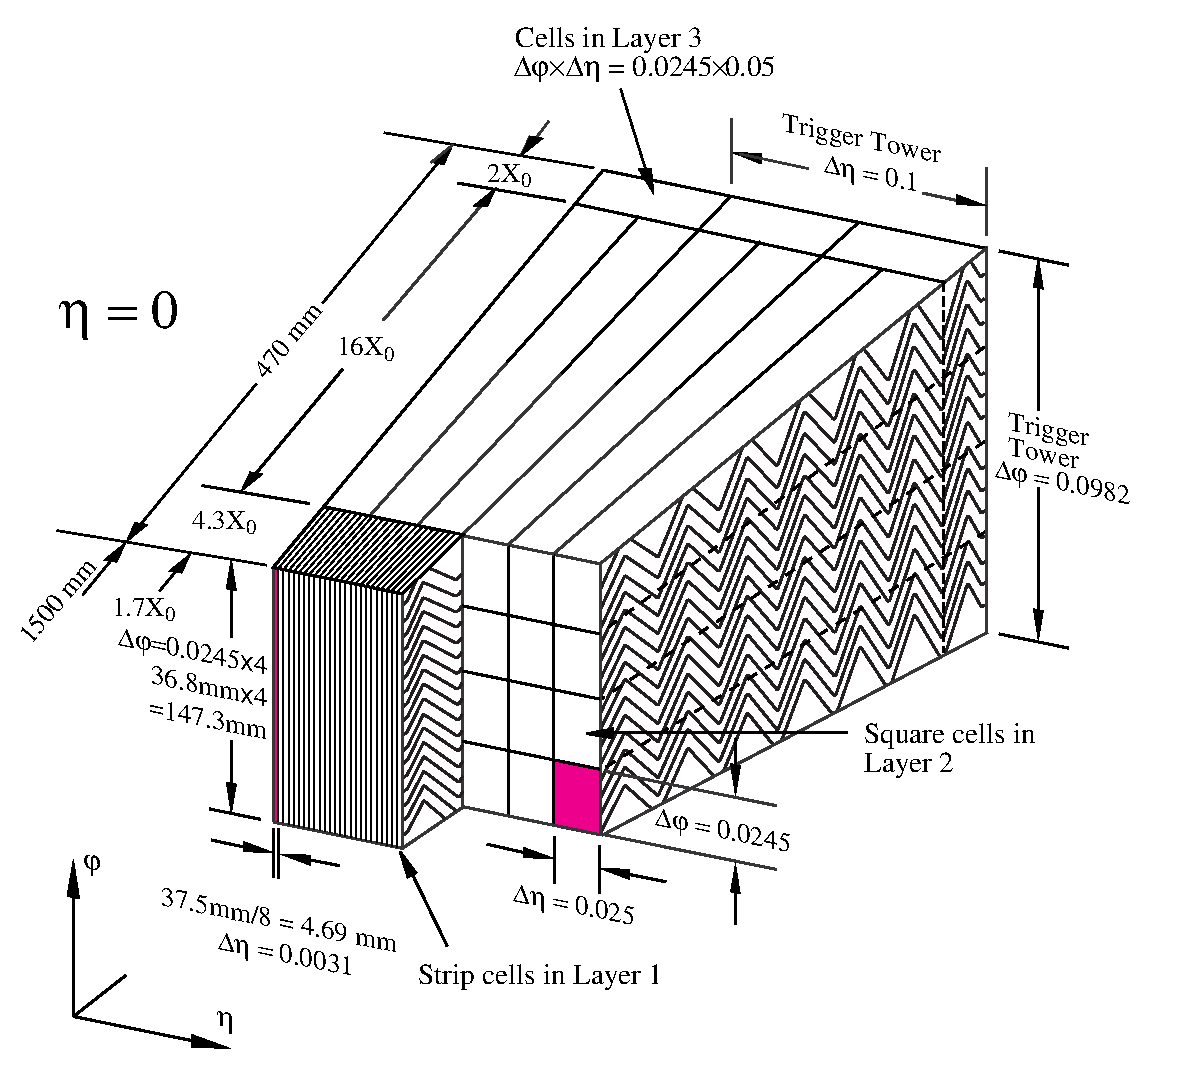
\includegraphics[width=0.8\linewidth]{figures/atlas/accordion}
    \caption{ \cite{PERF-2007-01} Sketch of LAr EMC barrel module where the lead
and liquid argon layers are visible in an accordion like geometry. Looking from
the foreground to the back there are 3 different types of cells visible.}
    \label{fig:accordion}
  \end{center}
\end{figure}

In the $|\eta| < 2.5$ region the EMC has 3 radial layers for precision physics
measurements.  Layer 1 consists of strip cells which are finely segmented with
$\Delta\eta = 0.0031$ and $\Delta\phi = 0.0245$ allowing for precision position
resolution which gives discrimination power between a single $\gamma$ deposit
and the $\pi^0$ characteristic $\gamma\gamma$ deposit. Layer 2 , which collects
the largest fraction of energy from electromagnetic shower, is segmented with
$\Delta\eta = .025$ and $\Delta\phi = 0.0245$. Layer 3 collects the tail of the
electromagnetic shower using a coarser segmentation of $\Delta\eta = .05$ and
$\Delta\phi = 0.0245$.  Additionally, in the region $|\eta| < 1.8$ a thin
pre-sampler , which contains no lead absorber, was placed in front of Layer 1 to
allow for energy corrections due to losses upstream of the EMC.  Combined the
EMC is $>$ 22 radiation lengths ($X_0$) in the barrel and $>$ 24 $X_0$ in the
end-caps, where a radiation length is the average distance an electron travels
in a given material before losing $1/e$ of its original energy $E_0$ via
bremsstrahlung radiation.

\subsection{Hadronic Calorimeter}

Directly outside the EMC envelope is the Hadronic Calorimeter (HCal) system
\cite{PERF-2007-01} which consists of three sampling calorimeter technologies:
the Tile calorimeter, the LAr hadronic end-cap calorimeter (HEC) and the LAr
forward calorimeter (FCal).  Combined, these three subsystems give measurements
of hadronic jet energies in the $0 <|\eta| < 4.9$ range. The tile calorimeter
uses steel as the absorber layer and scintillating tiles as the active material
and covers the region $|\eta| < 1.7$ with a barrel section flanked by two barrel
extensions each divided azimuthally into 64 modules.  These scintillator tiles
are read out on two sides by wavelength shifting fibers connected to
photomultiplier tubes as seen in \Cref{fig:tile_calorimeter}. At $\eta =
0$ the total tile calorimeter thickness is 9.7 nuclear interaction lengths
($\lambda$), where $\lambda$ is the average distance a hadron travels before
interacting inelastically with a nucleus.

\begin{figure}[!htbp]
  \begin{center}
    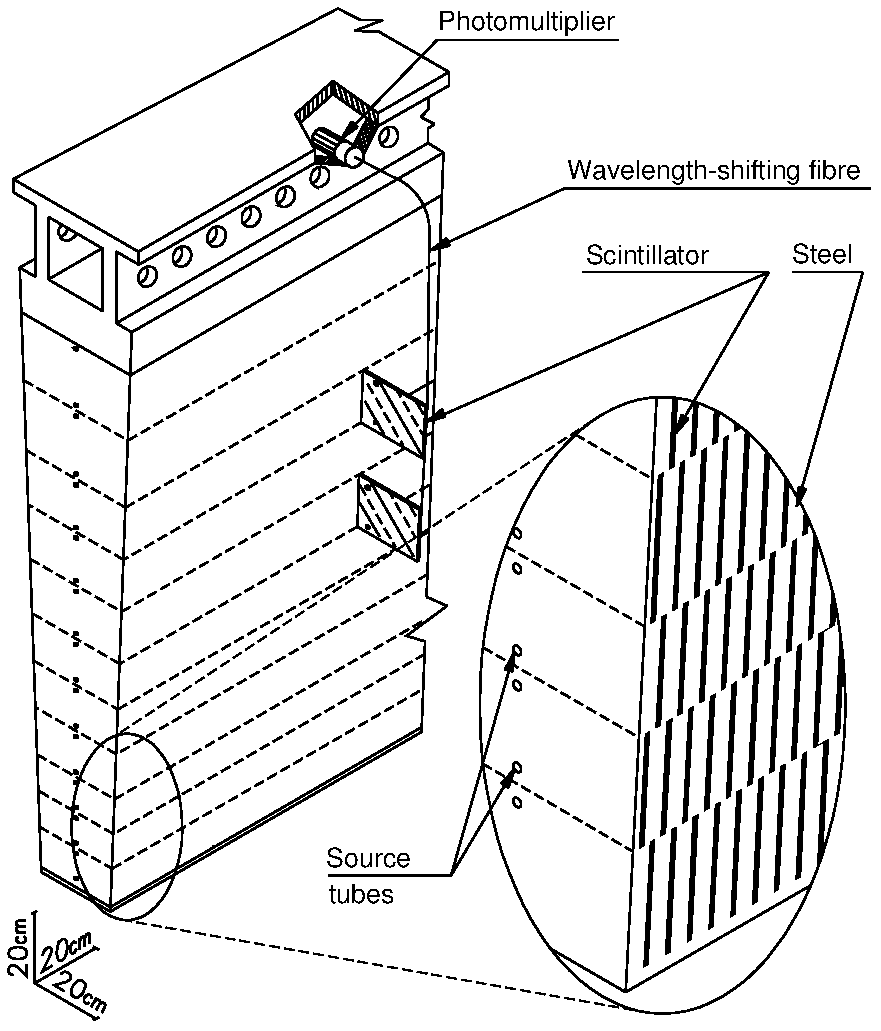
\includegraphics[width=0.8\linewidth]{figures/atlas/tile_calorimeter.pdf}
    \caption{ \cite{PERF-2007-01} Schematic of a tile calorimeter module
including a depiction of the connection between the scintillator tile to the
photomultiplier via a wavelength-shifting fibre.}
    \label{fig:tile_calorimeter}
  \end{center}
\end{figure}

The HEC is composed of two independent wheels per end-cap located just past the
EMC end-cap but sharing the same cryostat. This system  uses copper as an
absorber and liquid argon for the active material and covers the $1.5 < |\eta| <
3.2$ range using 32 wdge-shaped modules per wheel. Finally, the FCal shares the
same cryostat as the EMC and HEC end-caps and acts to extend the coverage of the
combined calorimeter system to include the $3.1 < |\eta| < 4.9$ range.  Each
endcap contains 3 modules, the first an electromagnetic module
(Copper/Liquid-Argon) which is followed by two hadronic modules which use
(Tungsten/Liquid-Argon).
